\documentclass[12pt]{article}
\usepackage[utf8]{inputenc}
\usepackage{float}
\usepackage{amsmath}
\usepackage{graphicx}

\usepackage[hmargin=3cm,vmargin=6.0cm]{geometry}
%\topmargin=0cm
\topmargin=-2cm
\addtolength{\textheight}{6.5cm}
\addtolength{\textwidth}{2.0cm}
%\setlength{\leftmargin}{-5cm}
\setlength{\oddsidemargin}{0.0cm}
\setlength{\evensidemargin}{0.0cm}




\begin{document}
Batyr Charyyev 2001527 Ceng-435 HW1 Report \\    
\\ 
\section*{1. Introduction}
Objections of our homework was to write basic packet based UDP socket application and conduct experiment with help of 'tc' command to calculate the end-to-end delay. Also we were familiarized with design of packet. 

\section*{2. Design}
We chose C language as a programming language. Our design was like node A(client) sends to node B(router) and it sends to C, C sends to D, D sends to E(server) via eth0(we consulted with assistant whether it will be problem to use eth0 and we get "it will not be problem as long as your program is stable") as an answer. We did not get any problems while we conducted experiments and we got reasonable results, so we continued with eth0. We get our data and IPs of all nodes through input.txt file. Our packet consist of header part and message part which ends with * character. 
\\In header we have index of source IP, index of destination IP and all IPs separeted by delimiter. Each packet that we sent was 70 bytes which includes header and message. When we sent last message server knows that it is last message from * character of our message and sends acknowledgement message back to client. From routing tables you can see how our nodes sent packets to other nodes.

Routing Tables

\begin{table}[h]
\small
	\centering 
	\caption{Routing Table A and Routing Table B}
	\label{table:example}
	\begin{tabular}{|c|c|c|c|}	%% specify column number
	\hline 							%% line draw	
	\textbf{Destination} & \textbf{Send To  } & \textbf{Destination} & \textbf{Send To}  \\
\hline 
\hline 
A & - & A & A   \\			%% rows distinguished with &
B & B & B & -    \\
C & B & C & C  \\
D & B & D & C  \\
E & B & E & C  \\

\hline 
\end{tabular}
\end{table}


\begin{table}[h]
\small
	\centering 
	\caption{Routing Table C and Routing Table D}
	\label{table:example}
	\begin{tabular}{|c|c|c|c|}	%% specify column number
	\hline 							%% line draw	
	\textbf{Destination} & \textbf{Send To  } & \textbf{Destination} & \textbf{Send To}  \\
\hline 
\hline 
A & B & A & C   \\			%% rows distinguished with &
B & B & B & C    \\
C & - & C & C  \\
D & D & D & -  \\
E & D & E & E  \\

\hline 
\end{tabular}
\end{table}

\begin{table}[h]
\small
\centering 
	\caption{ Routing Table for Node E }
	\label{table:example5}
	\begin{tabular}{|c|c|}	%% specify column number
	\hline 							%% line draw	
	\textbf{Destination} & \textbf{Send To}  \\
\hline 
\hline 
A & D   \\			%% rows distinguished with &
B & D    \\
C & D  \\
D & D  \\
E & -  \\

\hline 
\end{tabular}
\end{table}

In routing table of Node C if our packet has destination of A,B then it is send to B, if destination is D,E then it is send to D. In our code we determine our destination with help of sourceIndex and destinationIndex in header part of message. The implementation of it, is well clarified in ReadMe file. 




\section*{3. Implementation}

How to run the code and how the code works is provided in ReadMe file so I would like to skip this steps.

\section*{4. Experiment}
While we conducted experiments we used "tc"(traffic control) command to change emalutaion delay. Also we used "ntp"(network time protocol) to synchronize all nodes time.

\textbf{tc commands}:
\\ sudo tc qdisc add dev eth0 root netem delay 10ms   \quad\quad to add delay
\\ sudo tc qdisc change dev eth0 root netem delay 10ms \quad\quad to change delay
\\ sudo tc qdisc delete dev eth0 root netem \quad\quad\quad\quad\quad\quad\quad to delete delay

\textbf{ntp commands}:\\
$\quad $ $\quad $ sudo service ntp stop \quad\quad\quad \quad \quad \quad to stop ntp\\ 
sudo ntpdate -u 0.north-america.pool.ntp.org \quad to synchronize\\
$\quad $ $\quad $ sudo service ntp start \quad\quad\quad \quad \quad \quad to start ntp\\

results of our experiment is provided below\\
10 +- 5ms emaluation delay 42.8937ms end-to-end delay
\\20 +- 5ms emaluation delay 81.8760ms end-to-end delay
\\40 +- 5ms emaluation delay 166.58553ms end-to-end delay
\\80 +- 5ms emaluation delay 332.2583ms end-to-end delay




\begin{figure}[H]
\centering
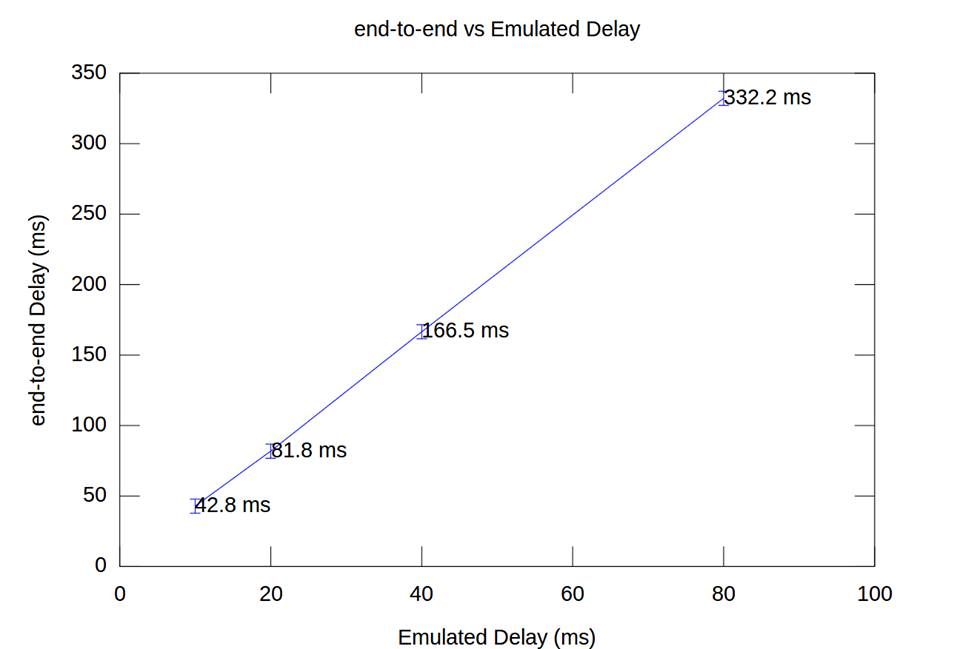
\includegraphics[width=140mm]{graph.jpeg}
\caption{A simple caption \label{overflow}}
\end{figure}

This graph shows the emaluation delay versus end-to-end-delay relation. We did the each experiment 10 times and took mean value of results. We can see that for 10ms emalutation delay we got 42.89ms end-to-end delay. From defintion of end-to-end delay which is:\\
 $ numberOfLinks *(propagationDelay+processingDelay+transmissionDelay)$
We can say that since we have four links it is reasonable for end-to-end delay to be 4 times larger than emalutaion delay.


\section*{5. Conclusion}
From definition of end-to-end delay, delay results because of transmission and propogation and proccessing parts also congestion in network results in different delays that is why we conducted experiment 10 times and took mean of it. The mean value is also as we expected. 
\\What can be changed? We analyse and change the header part of our message in every node which corresponds to processing delay so we can make it as minimum as possible to minimize our processing delay and end-to-end delay.




















\end{document}

​



